\documentclass[11pt]{article}
\usepackage{epsfig,psfrag}
\usepackage{amsmath}

\setlength{\textwidth}{6.2in}
\setlength{\oddsidemargin}{0.3in}
\setlength{\evensidemargin}{0in}
\setlength{\textheight}{8.7in}
\setlength{\voffset}{-.7in}
\setlength{\headsep}{26pt}
\setlength{\parindent}{10pt}
\begin{document}

%引用设置使用Bibtex
\usepackage{gbt7714}
\bibliographystyle{gbt7714-numerical}
%页面设置
\usepackage{geometry}
%字体设置
\usepackage{fontspec}
%\setmainfont{Times New Roman}
%定理环境
\usepackage{amsmath}
\numberwithin{equation}{section}
\usepackage{amsthm}
\newtheorem*{definition}{Definition}
\newtheorem{theorem}{Theorem}
\newtheorem{lemma}{Lemma}
\newtheorem*{corollary}{Corollary}
\newtheorem*{proposition}{Proposition}
\newtheorem*{example}{Example}
%数学环境字体
\usepackage{bm}
\usepackage[all]{xy}
%加载 TikZ 用于绘制交换图
\usepackage{tikz-cd}
\usepackage{tikz}
\usepackage{pgfplots}
\newcommand{\tikzdef}{\pgfmathsetmacro} % 在tikzpicture内的foreach循环中定义实数临时变量
%颜色
\usepackage{color,xcolor}

\definecolor{miku}{RGB}{57,197,187}
\definecolor{sakura}{RGB}{255,192,203}
\definecolor{rose}{RGB}{255,228,225}
\definecolor{brown}{RGB}{210,105,30}
\definecolor{lbrown}{RGB}{239,235,224}
\definecolor{bule}{RGB}{0,47,167}
\definecolor{lyellow}{RGB}{250,250,210}
\definecolor{lpurple}{RGB}{255,240,245}
\definecolor{lbule}{RGB}{135,206,250}
\definecolor{gbule}{RGB}{64,224,208}
\definecolor{green}{RGB}{138,200,207}
\definecolor{lgreen}{RGB}{225,255,255}
\definecolor{lorange}{RGB}{248,172,140}
\definecolor{salmon}{RGB}{250,128,114}
\definecolor{burgundy}{rgb}{0.5, 0.0, 0.13}
%链接设置
\usepackage[colorlinks=true,pdfstartview=FitH,linkcolor=blue,anchorcolor=violet, citecolor=magenta]{hyperref} 
%封面
\usepackage{pdfpages}
\usepackage{mathrsfs}
\usepackage{amssymb}
\usepackage{graphicx}
\usepackage{lipsum}
%彩色框
\usepackage{framed}
\usepackage{tcolorbox}
\tcbuselibrary{breakable}
\tcbuselibrary{theorems}
\tcbuselibrary{skins}
\usepackage{colortbl}
\usepackage{float}
\usepackage[export]{adjustbox}
\newtcolorbox[auto counter,number within=section]{notebox}[2][]{%
colback=miku!2!white,
colframe=miku,
coltitle=white,
fonttitle=\bfseries,
rightrule=2pt,
leftrule=2pt,
bottomrule=2pt,
colbacktitle=miku,
theorem style=standard,
breakable,
arc=2pt,
drop fuzzy shadow=black!20!white,
title=Note~\thetcbcounter: #2,#1}
\newtcolorbox[auto counter,number within=section]{markbox}[2][]{%
colback=miku!2!white,
colframe=miku,
coltitle=white,
fonttitle=\bfseries,
rightrule=0pt,
leftrule=0pt,
bottomrule=2pt,
colbacktitle=miku,
theorem style=standard,
breakable,
arc=0pt,
drop fuzzy shadow=black!20!white,
title=Remark~\thetcbcounter: #2,#1}
\newtcolorbox[no counter]{theorems}[2][]{%
width=12cm,
center,
sidebyside,
sidebyside adapt=left,
sidebyside gap=6mm,
sidebyside align=center seam,
colback=burgundy!2!white,
colframe=burgundy,
coltitle=white,
fonttitle=\bfseries,
rightrule=1pt,
leftrule=1pt,
bottomrule=2pt,
colbacktitle=burgundy,
theorem style=standard,
enhanced,
drop fuzzy shadow southeast=black!30!white,
breakable,
arc=0pt,
title=Theorem. #2,#1}
\newtcolorbox[no counter]{definitions}[2][]{%
width=12cm,
center,
colback=lyellow!2!white,
colframe=yellow!3!lyellow,
coltitle=bule,
fonttitle=\bfseries,
rightrule=0pt,
leftrule=1pt,
bottomrule=2pt,
colbacktitle=lyellow,
theorem style=standard,
breakable,
arc=5pt,
enhanced,
drop fuzzy shadow southeast=black!20!white,
title=Definition. #2,#1}
\newtcolorbox[auto counter,number within=section]{corollarys}[2][]{%
colback=lyellow!2!white,
colframe=lyellow,
coltitle=bule,
fonttitle=\bfseries,
rightrule=0pt,
leftrule=1pt,
bottomrule=2pt,
colbacktitle=lyellow,
theorem style=standard,
breakable,
arc=0pt,
enhanced,
drop fuzzy shadow southeast=black!20!white,
title=Corollary~\thetcbcounter: #2,#1}
\newtcolorbox[auto counter,number within=section]{lemmas}[2][]{%
width=12cm,
center,
colback=lyellow!2!white,
colframe=lorange!30!sakura,
coltitle=bule,
fonttitle=\bfseries,
rightrule=0pt,
leftrule=1pt,
bottomrule=2pt,
colbacktitle=lorange!30!sakura,
theorem style=standard,
breakable,
arc=5pt,
enhanced,
drop fuzzy shadow southeast=black!20!white,
title=Lemma. #2,#1}
\newtcolorbox[auto counter,number within=section]{propositions}[2][]{%
width=12cm,
center,
colback=salmon!5,
colframe=salmon!90!black,
coltitle=white,
fonttitle=\bfseries,
rightrule=1pt,
leftrule=1pt,
bottomrule=2pt,
colbacktitle=salmon!90!black,
theorem style=standard,
breakable,
arc=5pt,
enhanced,
drop fuzzy shadow southeast=black!20!white,
title=Proposition. #2,#1}
\newtcolorbox[no counter]{egbox}[2][]{%
width=12cm,
center,
colback=black!5!white,
colframe=black!20!white,
coltitle=black,
fonttitle=\bfseries,
rightrule=1pt,
leftrule=1pt,
bottomrule=2pt,
colbacktitle=black!20!white,
theorem style=standard,
breakable,
arc=0pt,
enhanced,
drop fuzzy shadow southeast=black!20!white,
title=Example. #2,#1}

%\begin{figure}[H]
%\centering
%\includegraphics[center]{pic.png}
%\end{figure}
\geometry{left=3cm,right=3cm,top=2cm,bottom=2cm}
\tcbuselibrary{most}

\usepackage[linesnumbered,ruled,vlined]{algorithm2e}
\usepackage{algorithmic}

\SetKwProg{Fn}{function}{\string:}{}
\newcommand{\forcond}{$i=0$ \KwTo $n$}
\SetKwFunction{FRecurs}{FnRecursive}
\SetKwInput{KwCost}{Cost}

\usepackage{holtpolt}

%自定义设置
\renewcommand{\proofname}{Proof.}
\renewcommand{\contentsname}{ Content }
\newcommand{\image}[2]{
    \centering
    \includegraphics[width={#1}\textwidth]{#2}
}



\newcommand\keywords[1]{\vskip2ex\par\noindent\normalfont{\textbf{关键词}: #1}}
\newcommand{\ekeywords}[1]{\vskip2ex\par\noindent\normalfont{\bfseries Key Words: }#1}
\newcommand{\miku}{\textcolor{miku}}
\newcommand{\sakura}{\textcolor{sakura}}
\newcommand{\brown}{\textcolor{brow}}
\newcommand{\red}{\textcolor{red}}
\newcommand{\blue}{\textcolor{blue}}
\newcommand{\A}{\mathcal{A}}
\newcommand{\C}{\mathbb{C}}
\newcommand{\al}{\alpha}
\newcommand{\sa}{$\sigma$-algebra}
\newcommand{\Bsa}{Borel $\sigma$-algebra}
\newcommand{\F}{\mathcal{F}}
\newcommand{\N}{\mathcal{N}}
\newcommand{\M}{\mathcal{M}}
\newcommand{\m}{ $\mathcal{M}$ }
\newcommand{\B}{\mathcal{B}}
\newcommand{\myP}{\mathcal{P}}
\renewcommand{\bf}[1]{\textbf{#1}}

\newcommand{\myRom}[1]{\uppercase\expandafter{\romannumeral#1}}
\newcommand{\pl}{$ L^p(X) $}
\newcommand{\twol}{$ L^2(X) $}
  % input some useful macros

% Macros for exercises:

\newcommand{\exernum}{0.0} % will be set to current Exercise number

% Headers:

\newcommand{\exercise}[2][\null]{\vskip 15pt \noindent%
     {\large \bf Exercise #2}~ {\it #1}%
     \nopagebreak\vskip 5pt \nopagebreak%
     \renewcommand{\exernum}{#2} \setcounter{equation}{0}%
     \addcontentsline{toc}{subsection}{Exercise #2 \hskip 5pt #1}}
     % \exercise has optional first argument -- short descriptor
     % the exercise number is stored in \exernum for use in labeling equations

\newcommand{\chapexercises}[1]{%
     \cleardoublepage
     \centerline{\LARGE\bf Chapter #1 Exercises}
     \vskip .5cm
     \noindent
     From: {\it Finite Difference Methods for Ordinary and Partial 
     Differential Equations}\\  by R.~J.~LeVeque, SIAM, 2007.~~~
     {\tt http://www.amath.washington.edu/$\sim$rjl/fdmbook}
     \vskip .5cm
     \addcontentsline{toc}{section}{Chapter #1}
     }

% Parts:

% set enumerate to give parts a, b, c, ...  rather than numbers 1, 2, 3...
\renewcommand{\theenumi}{\alph{enumi}}
\renewcommand{\labelenumi}{(\theenumi)}

% set second level enumerate to give parts i, ii, iii, iv, etc.
\renewcommand{\theenumii}{\roman{enumii}}
\renewcommand{\labelenumii}{(\theenumii)}

% Equations:

% label equations starting with E for exercise, then exernum, then a,b,c etc
\renewcommand{\theequation}{Ex\exernum\alph{equation}}


% commands for labeling and citing equations to add exernum automatically.
%   then set equations using e.g. \eqlex{a} ... \end{equation}
%   and cite as \eqnex{a}
\newcommand{\eqlex}[1]{\begin{equation}\label{\exernum #1}}
\newcommand{\eqnex}[1]{(\ref{\exernum #1})}
       % more macros for exercise formatting

% For exercises,
% set enumerate to give parts a, b, c, ...  rather than numbers 1, 2, 3...
\renewcommand{\theenumi}{\alph{enumi}}
\renewcommand{\labelenumi}{(\theenumi)}


% header:
\chapexercises{4}


\exercise[(Convergence of SOR)]{4.1}

The m-file \verb+iter_bvp_Asplit.m+ implements the Jacobi, Gauss-Seidel, and
SOR matrix splitting methods on the linear system arising from the boundary
value problem $u''(x) = f(x)$ in one space dimension.  

\begin{enumerate}
\item Run this program for each method and produce a plot similar to 
Figure~4.2.

\item The convergence behavior of SOR is very sensitive to the choice of
$\omega$ ({\tt omega} in the code).  Try changing from the optimal $\omega$
to $\omega = 1.8$ or 1.95.

\item Let $g(\omega) = \rho(G(\omega))$ be the spectral radius of the
iteration matrix $G$ for a given value of $\omega$.  Write a program to
produce a plot of $g(\omega)$ for $0\leq \omega \leq 2$.

\item From equations (4.22) one might be tempted to try to implement SOR as
\begin{verbatim}
     for iter=1:maxiter
        uGS = (DA - LA) \ (UA*u + rhs);
        u = u + omega * (uGS - u);
        end
\end{verbatim}
where the matrices have been defined as in \verb+iter_bvp_Asplit.m+.
Try this computationally and observe that it does not work well.  Explain
what is wrong with this and derive the correct expression (4.24).

\end{enumerate} 


\exercise[(Forward vs.\ backward Gauss-Seidel)]{4.2}

\begin{enumerate}
\item The Gauss-Seidel method for the discretization of $u''(x) = f(x)$
takes the form (4.5) if we assume we are marching forwards across the grid,
for $i=1,~2,~\ldots,~m$.  We can also define a {\it backwards Gauss-Seidel
method} by setting
\eqlex{a}
u_i^{[k+1]} = \half (u_{i-1}^{[k]} + u_{i+1}^{[k+1]} - h^2 f_i), \qquad
\text{for}~ i = m,~m-1,~m-2,~\ldots,~1.
\end{equation}
Show that this is a matrix splitting method of the type described in
Section~4.2 with $M = D-U$ and $N=L$.

\item Implement this method in \verb+iter_bvp_Asplit.m+ and observe that it
converges at the same rate as forward Gauss-Siedel for this problem.

\item Modify the code so that it solves the boundary value problem
\eqlex{b}
\epsilon u''(x) = au'(x) + f(x),\qquad 0\leq x \leq 1,
\end{equation} 
with $u(0) = 0$ and $u(1) = 0$, where $a\geq 0$ and the $u'(x_i)$ term
is discretized by the one-sided approximation $(U_i - U_{i-1})/h$.
Test both forward and backward Gauss-Seidel for the resulting linear system.
With $a=1$ and $\epsilon = 0.0005$.  You should find that they behave very
differently:

\psfrag{forwardGS}{forward}
\psfrag{backwardGS}{backward}
\hfil\epsfig{file=figs/iter_bvp_advdiff.eps,width=3.5in}\hfil

Explain intuitively why sweeping in one direction works so much better than
in the other.

{\bf Hint:} Note that this equation is the steady equation for an 
advection-diffusion
PDE $u_t(x,t) + au_x(x,t) = \epsilon u_{xx}(x,t) - f(x)$.  
You might consider how the methods behave in the case $\epsilon = 0$.
\end{enumerate} 


\end{document}


